\section{Исследовательская часть}

В данном разделе приведены технические характеристики устройства, на котором проводилось измерение времени работы программного обеспечения, а также результаты замеров времени.

\subsection{Постановка эксперимента}

Целью эксперимента является провести анализ скорости работы алгоритма генерации изображения с использованием алгоритма Z-буфером.

\subsubsection{Технические характеристики}

Технические характеристики устройства, на котором выполнялось тестирование.
\begin{itemize}
	\item Процессор: Intel(R) Core(TM) i5-10300H CPU 2.50 ГГц~\cite{intel}.
	\item Количество ядре: 4 физических и 8 логических ядер.
	\item Оперативная память: 16 ГБайт.
	\item Операционная система: Windows 11 Pro 64-разрядная система~\cite{windows}.
\end{itemize}

Тестирование проводилось на стационарном компьютере. Во время тестирования устройство было нагружено только встроенными приложениями окружения, а также непосредственно системой тестирования.

\subsubsection{Результаты эксперимента}

Для исследования зависимости времени тренинга изображения от числа объектов на сцене, использовались объекты с фиксированным числом граней, каждый объект имел освещенную и затененную части. Количество объектов менялось на сцене от 100 до 1000 с шагом 100, были рассмотрены случаи для 3-х, 6-ти и 9-тигранных объектов. Результаты проведенного исследования представлены.

\begin{figure}[h]
	\centering
	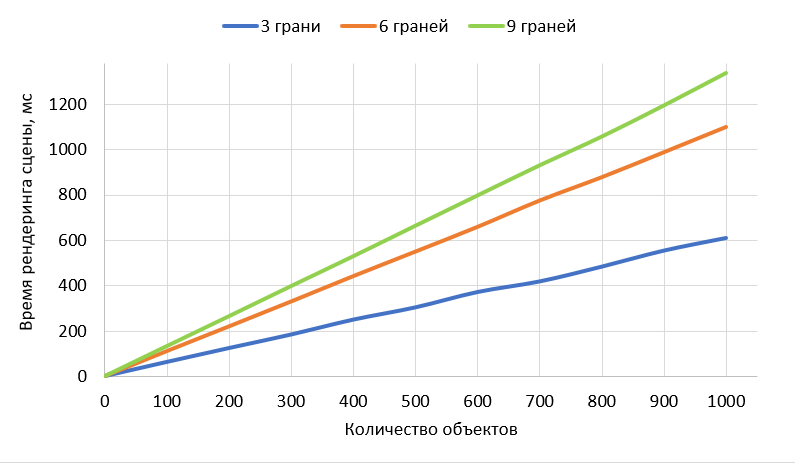
\includegraphics[width=0.9\textwidth]{img/exp/exp1.png}
	\caption{График зависимости времени отрисовки от числа объектов}
	\label{fig:exp-1}
\end{figure}

Как видно из графика, время рендеринга сцены зависит от количества объектов линейно, независимо от числа их боковых граней.

Следующим этапом исследования разработанной программы является исследование зависимости времени построения сцены от числа боковых граней объектов при фиксированном количестве объектов. В ходе эксперимента количество боковых граней менялось от 50 до 500 с шагом 50, при этом были рассмотрены случаи для 2-х объектов с равным числом граней и для 2-х объектов, у одного из которых число граней менялось, а у другого было фиксировано. 

\begin{figure}[h]
	\centering
	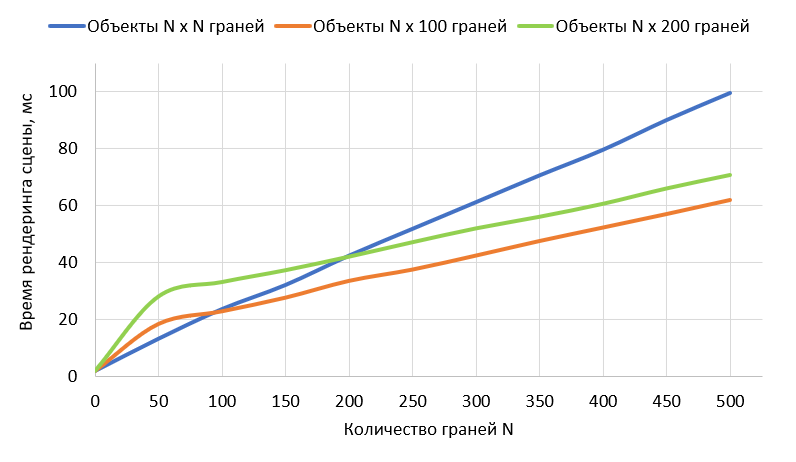
\includegraphics[width=0.9\textwidth]{img/exp/exp2.png}
	\caption{График зависимости времени отрисовки от числа боковых граней}
	\label{fig:exp-2}
\end{figure}

Из проведенного эксперимента можно сделать вывод, что время рендеринга сцены линейно зависит от числа боковых граней объектов, при этом для 2-х объектов время растет вдвое быстрее, если количество граней у обоих увеличивается одновременно, чем в случае фиксированного количества граней у одного из них. В случаях фиксированного количества граней время растет одинаково, постоянная разница во времени объясняется разным числом граней у фиксированного объекта.

\subsection*{Вывод}
В данном разделе приведены результаты работы программного
обеспечения и проведен эксперимент с использованием библиотеки time,
функции которой использовались для определения эффективности работы
программы по времени.

Результаты эксперимента совпали с ожидаемыми, так как в ходе
эксперимента было установлено, что время работы увеличивается с увеличением
количества объектов на сцене и количеством ребер у объекта.